
There are several ways to formulate the trust of text appearing
in an article.
Possibilities include directly ascribing the reputation
of the author to the text,
using a citation-based trust system
(\eg PageRank~\cite{PageRank98,Kleinberg99}),
and ratings systems such those used in
Amazon\footnote{Users are asked whether individual reviews
are ``helpful;'' the tally of these ratings
describes the trust the community places in the review.}
and Slashdot.\footnote{Users rate each other's comments as positive
or negative, with weighting based on the commenter's reputation.}
Each of these ideas assigns a trust to the whole article,
but this isn't the right granularity of text for a project
where articles are constantly being revised and vandalized.
\begin{comment}
For example, the Wikipedia's \textit{featured article} status is
another ``whole article'' trust metric, reserved
for high quality articles which the community votes for, but 
which is occasionally removed through another vote
when the article falls into disrepair.
This manual process allows a time lag during which
an article is in disrepair but users are not aware
of the tarnished status.
\end{comment}


Some smaller granularity than a whole article seems more
appropriate when the entire article is subject to potential
revision at any moment.
The idea of tracking \textit{fragments} of text introduced in
the same version was proposed in~\cite{McGuinness06}, but
this still assumes a uniform level of trust for the portion
of a fragment which is preserved.
We propose that assigning trust to individual words best
captures the dynamic that some portions of contributions will be
contentious and require more editing before reaching community concensus.
Our solution, guided by the idea of preserving the
current user experience, considers edits to an
article as an implicit statement about the existing content:
deleting text is a vote against that text, while preserving
text is a vote in favor of the text.
As more people edit a document, the portions which remain
the same in each version become increasingly more trustworthy.

There are two significant problems with a simple
``more review means more trustworthy'' model, however.
The more intuitive problem is that \intro{author attention}
is not uniform.
That is, when an author makes an edit to
a large article, she will most often focus her attention only
on the region containing her edit; preserving text in
other portions of the article are not quite a full vote
that they are trustworthy.
The other problem is in relating the trust information to
a user: the Wikipedia is constantly being revised, and
some pages (\eg the page for George W. Bush) would always
be entirely at the lowest trust level because there is so much
vandalism.
Users would not have a useful view of such pages, and
are apt to ignore trust information if too much
text is flagged as untrustworthy.
Our research~\cite{WikiTrust2008} attempts to address these
issues and presents the trust information to users
by coloring the background of the article text
(see Figure~\ref{fig-trust-ex} for an example).

\begin{figure}[t]
\centering
\framebox{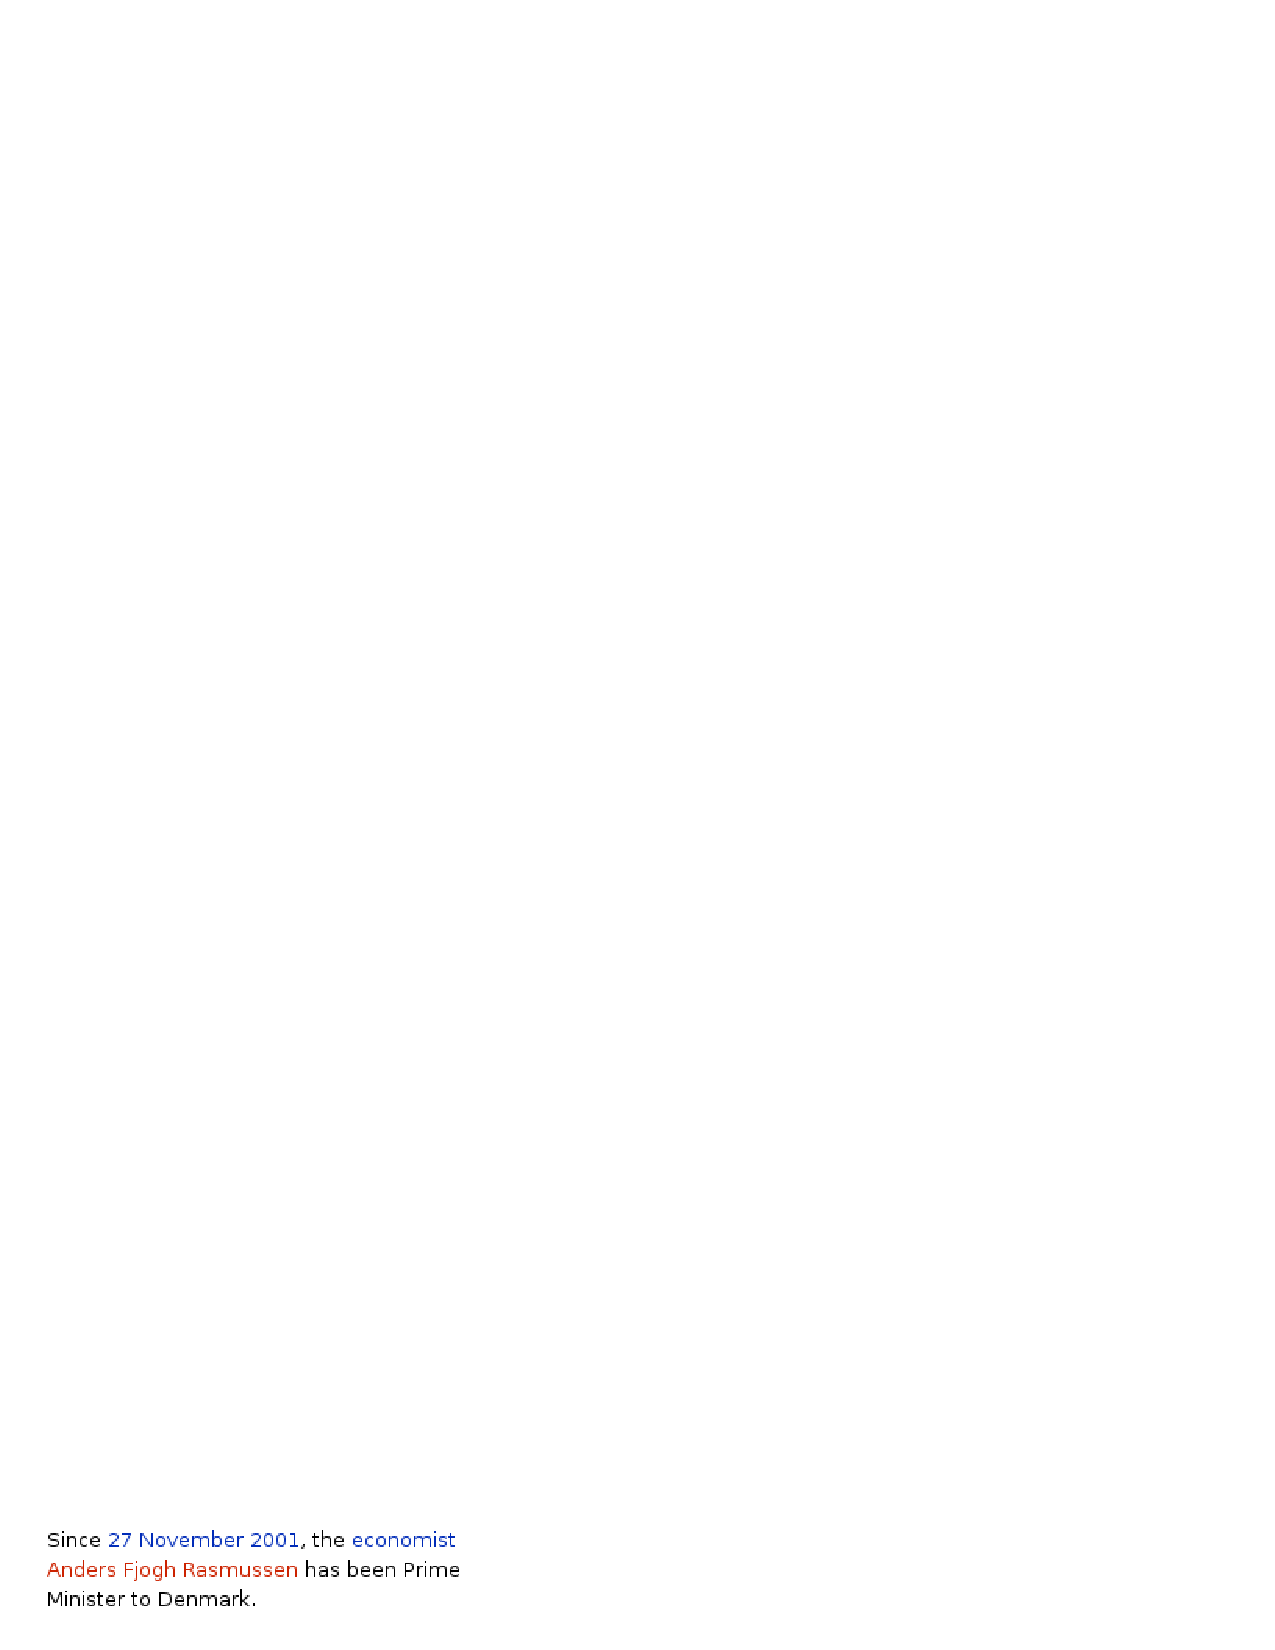
\includegraphics[width=0.55\textwidth]{part-C10-intro/Denmark-Fjogh}}
\caption{A trust colorized version of Figure~\ref{fig-denmark}.
    The darker orange the background, the less trustworthy
    the text.
    Notice that the shade gets lighter with increasing distance
    from the location of the change.}
\label{fig-trust-ex}
\end{figure}

	\mynote{Fix the image!}

